\section{\CChell{}: Accelerating Legacy Storage with NVMM}
\label{sec:overview}

\DAChell{} is useful if the entire file system resides in NVMM, but many
storage systems are too large to fit in NVMM.  To improve
performance of these systems, \Chell{} provides an alternative mode of
operation called \CChell{}.  \CChell{} uses NVMM to provide a reliable,
consistent, write-back cache of data that resides in an existing file system.
\CChell{} provides fast access to the cached data using the same techniques
that \DAChell{} uses but it accesses cached data rather than actual file data.
This section and the next describe the differences between \CChell{} and \DAChell{}.

Figure~\ref{fig:CChellstack} shows the system architecture of \CChell{}.
Like \DAChell{}, there is an userspace library, \lib{} to handle cache
hits, but \CChell{} also adds a kernel module, \drv{}, to
manage the contents of the cache and interact with the file system on the
backing store device.

The only difference in \libd{} and \lib{} is in
how they detect and react to a miss.  \Libd{} detects a miss when it
finds that its B-tree does not contain an entry for the file location the
application is trying to access.  This occurs the first time the application
accesses each chunk.  Its response is simple, issues an \texttt{mmap()} to map the chunk.

\Lib{} can also experience a miss when an entry is missing from its B-tree.
But a miss can also manifest itself as a segmentation fault, if the data was
mapped into userspace but the kernel had to evict it to make room for other data.
In both cases, \lib{} issues an \texttt{ioctl()} to \drv{} requesting that
it load the data from the backing store (if needed), and then map the data into
the application's address space.

\Drv{} manages the data cached in the NVMM.
It copies data between cache pages and the backing store device,
memory maps the requested cache pages to the application's address space,
and handles cache write back and eviction.

When \drv{} receives the \texttt{ioctl} request from \lib{},
it first checks the
file Inode permission to make sure it is a valid request.  Then it checks if 
the requested data is in the cache,
and loads it, if required.
Next, \drv{} copies data from the user buffer to the cache pages if it is
a write, or from the backing store device to the cache pages and user buffer if 
it is a read. Then it calls \texttt{mmap()} to map the cache pages to
the application's address space and returns the mapped address and length
to \lib{}.

%\cfigure[Figures/Chell-Stack.pdf,{\figtitle{\CChell{} system stack}},fig:CChellstack]

\begin{figure}
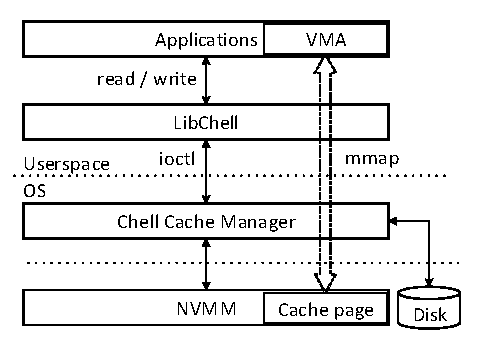
\includegraphics{Figures/Chell-Stack.pdf}
\caption{\CChell{} architecture: \CChell{} caches files stored on slow storage
devices in NVMM, provides a fast, POSIX-compliant interface to applications.}
\label{fig:CChellstack}
\end{figure}

%\cfigure[Figures/Chell-Stack.pdf,{\figtitle{\CChell{} architecture}: by combining NVMM with the ability to map files into userspace, \DAChell{} provides applications with a fast, POSIX-compliant interface to data stored in NVMM. fig

%%%%%%%%%%%%%%%%%%%%%%%%%%%%%%%%%%%%%%%%%%%%%%%%%%%%%%%%%%%%%%%%%%%%%%%%%%%%%%%%%%%%%%
%%%%%%%%%%%%%%%%%%%%%%%%%%%%%%%%%%%%%%%%%%%%%%%%%%%%%%%%%%%%%%%%%%%%%%%%%%%%%%%%%%%%%%
%%%%%%%%%%%%%%%%%%%%%%%%%%%%%%%%%%%%%%%%%%%%%%%%%%%%%%%%%%%%%%%%%%%%%%%%%%%%%%%%%%%%%%
%%%%%%%%%%%%%%%%%%%%%%%%%%%%%%%%%%%%%%%%%%%%%%%%%%%%%%%%%%%%%%%%%%%%%%%%%%%%%%%%%%%%%%
%%%%%%%%%%%%%%%%%%%%%%%%%%%%%%%%%%%%%%%%%%%%%%%%%%%%%%%%%%%%%%%%%%%%%%%%%%%%%%%%%%%%%%
%%%%%%%%%%%%%%%%%%%%%%%%%%%%%%%%%%%%%%%%%%%%%%%%%%%%%%%%%%%%%%%%%%%%%%%%%%%%%%%%%%%%%%
%%%%%%%%%%%%%%%%%%%%%%%%%%%%%%%%%%%%%%%%%%%%%%%%%%%%%%%%%%%%%%%%%%%%%%%%%%%%%%%%%%%%%%

\ignore{
For each file cached in \CChell{}, there is a non-volatile file descriptor (NVfd)
data structure in \lib{}, and a non-volatile inode (NVnode) data structure represents the Inode.
When an application opens a file with \texttt{open()}, \lib{} allocates
a new NVfd and either allocates a new NVnode or uses an existing NVnode,
depending on whether the file has been opened previously.

\Lib{} intercepts most POSIX system calls and handles them internally.
For example,
\texttt{lseek()} updates the file offset in NVfd, and \texttt{dup()} and \texttt{dup2()}
make a NVfd alias to another NVfd.
}

\ignore{For each file Inode cached in \CChell{},
there is a cache extent tree to store the cached file extents
\texttt{mmap} information. The key is the file offset,
and the value is the mapped address and length. When application
triggers \texttt{read()} and \texttt{write()} calls to the file Inode,
\lib{} lookups the tree to check if the required extent is cached.
If it's a cache hit,
\lib{} simply uses \texttt{memcpy()} to transfer data between application
buffers and the memory mapped cache pages, thereby satisfying the request
without entering the kernel.}

\ignore{If the extent is not cached in the tree, it's a cache miss. In this case,
\lib{} sends the request to \drv{} via an \texttt{ioctl()} call.
\drv{} then serves the request by allocating new cache pages, transferring
data between application buffers and
the cache pages, and then memory mapping the cache pages to the application's
address space. The mapped address and length are returned to \lib{},
which inserts the extent into the corresponding cache extent tree. When this extent is accessed again,
it will be a cache hit and \lib{} will serve it with \texttt{memcpy}.}

By default \CChell{} requires all the applications to access the NVMM cache via
\lib{}.  Otherwise, if one application accesses a cached file via \CChell{}, while another
application accesses the same file on the backing store device via POSIX write,
\CChell{} and the file system on the backing store device will have an
inconsistent view about the file.  To prevent this inconsistency, \drv{}
interposes at the block device driver for the backing store and rejects
accesses that touch cached data but that are not from applications using \lib{}.

\ignore{ \lib{} forwards metadat changes to \drv{}, and
\drv{} 

 In this mode \lib{} does not
issue POSIX requests for file metadata change; instead it sends all the requests
that write to the backing store device to \drv{}.
\drv{} only accepts requests from \lib{}, and it records all the valid requests.
If it receives request to write to backing store device but is not recorded, it
will simply reject the request. In this mode \CChell{} guarantees all the applications
access NVMM cache via \lib{}.

}
